\chapter{Metodologia}
\label{cap:metodologia}

Neste capítulo, defino os procedimentos que pretendo utilizar para evoluir, documentar e avaliar o protótipo Estoque Fácil em correspondência com o problema apresentado na introdução. Como este documento corresponde ao TCC I, apresento a implementação complementar, os testes e a análise como planejamento para o TCC II. Distingo a consulta documental que realizo nesta etapa da avaliação futura de uma versão identificada do sistema.

\section{Caracterização da pesquisa}

Caracterizo minha pesquisa como aplicada porque direciono a produção de conhecimento a um problema de controle de estoques e ao desenvolvimento de uma solução de software. Quanto aos objetivos, adoto caráter exploratório para identificar necessidades e alternativas e caráter descritivo para documentar requisitos, arquitetura e comportamento observado. No TCC II, combinarei a análise qualitativa de documentos e decisões com medidas quantitativas descritivas dos testes.

Adotarei como procedimento central um estudo de caso único, delimitado ao Estoque Fácil. Organizo o protocolo segundo as etapas de planejamento, preparação da coleta, obtenção de evidências, análise e relato discutidas por \citeonline{RunesonHost2009}. Utilizo pesquisa bibliográfica e documental para fundamentar e analisar o caso e pretendo empregar desenvolvimento incremental nas alterações definidas para o TCC II. Não pretendo realizar um levantamento estatisticamente representativo do mercado regional.

\section{Objeto, unidade de análise e delimitação}

Adoto como objeto o protótipo web Estoque Fácil, identificado pelo repositório de software de \citeonline{EstoqueFacilRepositorio}. Defino como unidade de análise a relação entre requisitos selecionados, decisões de implementação e evidências de verificação. No TCC I, examino código-fonte, documentação, modelo de dados e configurações; no TCC II, acrescentarei registros de mudanças e resultados dos testes.

Delimito o núcleo funcional a usuários e permissões, produtos, categorias, fornecedores, entradas, saídas, consulta de saldo, histórico e relatórios. Incluirei nos cenários de avaliação o vínculo da saída a setor e funcionário e a visualização por setor. Testarei lotes, inventários e recursos multiempresa quando integrarem os fluxos da versão selecionada. Não incluirei vendas, emissão de documentos fiscais, contabilidade ou otimização de compras como exigências deste estudo.

Na inspeção funcional deste capítulo, utilizo uma cópia local do repositório do Estoque Fácil, consultada em 16 de setembro de 2026 \cite{EstoqueFacilRepositorio}. Como o protótipo permanece em desenvolvimento, essa inspeção representa um recorte do código, e não uma versão final do sistema. Antes da avaliação do TCC II, produzirei uma versão identificável que reúna código, documentação e configuração e registrarei eventuais diferenças locais. Vincularei a avaliação a essa versão, e não ao estado mutável da branch principal.

\subsection{Estado inicial e contribuição prevista}
\label{sec:estado-contribuicao}

Na Tabela~\ref{tab:estado-contribuicao}, delimito a contribuição acadêmica em relação ao protótipo que desenvolvi antes e durante o TCC I. ``Presente no protótipo'' indica código ou configuração que identifiquei por inspeção, sem representar aprovação em testes. ``A corrigir no TCC II'' identifica uma divergência já observada; ``a desenvolver no TCC II'' reúne artefatos e complementações previstos; e ``a avaliar no TCC II'' designa comportamentos cujo atendimento ainda precisarei demonstrar. Um mesmo módulo poderá estar presente no protótipo e ainda depender de avaliação.

\begin{table}[htb]
\centering
\caption{Estado inicial do protótipo e contribuição prevista no TCC}
\label{tab:estado-contribuicao}
\small
\begin{tabular}{p{0.17\textwidth}p{0.36\textwidth}p{0.36\textwidth}}
\hline
\textbf{Estado} & \textbf{Objeto e evidência inicial} & \textbf{Entrega ou condição de conclusão} \\ \hline
Presente no protótipo & Rotas e serviços de cadastros, entradas, saídas, relatórios e painel por setor. & Inventariar os recursos e vinculá-los aos requisitos, sem apresentá-los como implementação nova do TCC. \\ \hline
Presente no protótipo & Modelos SQLAlchemy, arquivos Compose e serviços de inventário, lotes, reposição e backup. & Registrar a versão e documentar as responsabilidades e limitações encontradas. \\ \hline
A corrigir no TCC II & Gatilho do workflow referencia \texttt{develop}, enquanto o fluxo proposto utiliza \texttt{developer}. & Alinhar a configuração e registrar uma execução do fluxo na branch definida. \\ \hline
A desenvolver no TCC II & Etapas explícitas de testes no pipeline e organização da base experimental com PostgreSQL. & Entregar configuração versionada, dados sintéticos e evidência de execução automatizada. \\ \hline
A desenvolver no TCC II & Matriz de rastreabilidade, casos de teste e registros de decisões; complementações decorrentes de falhas verificadas. & Relacionar requisito, alteração, teste e resultado; justificar mudanças de escopo. \\ \hline
A avaliar no TCC II & Saldo, concorrência, permissões, vínculos de retirada, filtros por setor, desempenho e recuperação de backup. & Produzir relatório com resultados positivos, falhas, casos bloqueados e limitações. \\ \hline
\end{tabular}
\par\smallskip
{\footnotesize Fonte: elaboração própria a partir da inspeção de \cite{EstoqueFacilRepositorio} em 16 set. 2026.}
\end{table}

Apresento os diagramas e o levantamento documental a seguir como artefatos iniciais do TCC I. Antes das alterações planejadas para o TCC II, preservarei a base de comparação por meio do commit e das diferenças locais pertinentes. No relatório final, descreverei apenas as mudanças realizadas após essa base e as associarei aos registros de desenvolvimento. Falhas ainda não demonstradas, como uma possível inconsistência sob concorrência, permanecerão classificadas como itens a avaliar; sua correção somente será contabilizada se houver evidência do problema e da mudança correspondente.

\subsection{Visão da arquitetura existente}

Na Figura~\ref{fig:arquitetura-estoque}, sintetizo o fluxo que identifiquei em \path{app/main.py}, nas rotas, nos serviços e em \path{app/database.py}. A aplicação gera HTML no servidor, utiliza serviços de negócio e também contém consultas realizadas diretamente pelas rotas. Portanto, o diagrama não pressupõe separação estrita entre todas as camadas. Sessão e permissões são tratadas na aplicação; o desenho representa responsabilidades lógicas e não serviços independentes.

\begin{figure}[htb]
\centering
\begin{tikzpicture}[>=stealth, every node/.style={font=\small}, box/.style={draw,rounded corners,align=center,minimum height=1cm,text width=5.2cm,fill=blue!4}, node distance=0.8cm]
\node[box] (browser) {Navegador\\Formulários, consultas e relatórios};
\node[box,below=of browser] (routes) {FastAPI / Uvicorn\\Rotas, sessão e permissões};
\node[box,below=of routes] (services) {Serviços de negócio\\Movimentações, inventário e reposição};
\node[box,below=of services] (orm) {SQLAlchemy\\Modelos, sessões e consultas};
\node[box,below=of orm] (db) {Banco relacional\\PostgreSQL no protocolo experimental};
\node[draw,rounded corners,align=center,text width=3cm,right=1.5cm of routes,fill=gray!8] (templates) {Jinja2 + Bootstrap\\Geração de HTML};
\draw[<->] (browser) -- node[right,font=\footnotesize] {HTTP / HTML} (routes);
\draw[->] (routes) -- (services);
\draw[->] (services) -- (orm);
\draw[<->] (orm) -- (db);
\draw[<->] (routes) -- (templates);
\draw[->,dashed] (routes.west) -- ++(-0.65,0) |- node[pos=0.7,left,font=\footnotesize,align=right] {consultas diretas\\em algumas rotas} (orm.west);
\end{tikzpicture}

\caption{Visão lógica da aplicação e configuração de banco prevista para a avaliação}
\label{fig:arquitetura-estoque}
\par\smallskip
{\footnotesize Fonte: elaboração própria a partir de \cite{EstoqueFacilRepositorio}.}
\end{figure}

PostgreSQL é o banco escolhido para o ambiente experimental. A possibilidade de SQLite na configuração local preexistente permanece explicitada na análise tecnológica. Proxy reverso, publicação de imagens e servidor de hospedagem pertencem à visão de implantação discutida no Capítulo~\ref{cap:referencial} e não estão representados nesta figura.

\subsection{Recorte do modelo de dados}

Na Figura~\ref{fig:dados-estoque}, apresento um recorte do modelo relacional que construí a partir das classes SQLAlchemy de produto, categoria, movimentação, usuário, setor, fornecedor e funcionário. PK identifica chave primária e FK, chave estrangeira. As multiplicidades próximas a cada entidade indicam quantas instâncias dela podem estar associadas a uma instância da entidade oposta.

\begin{figure}[htb]
\centering
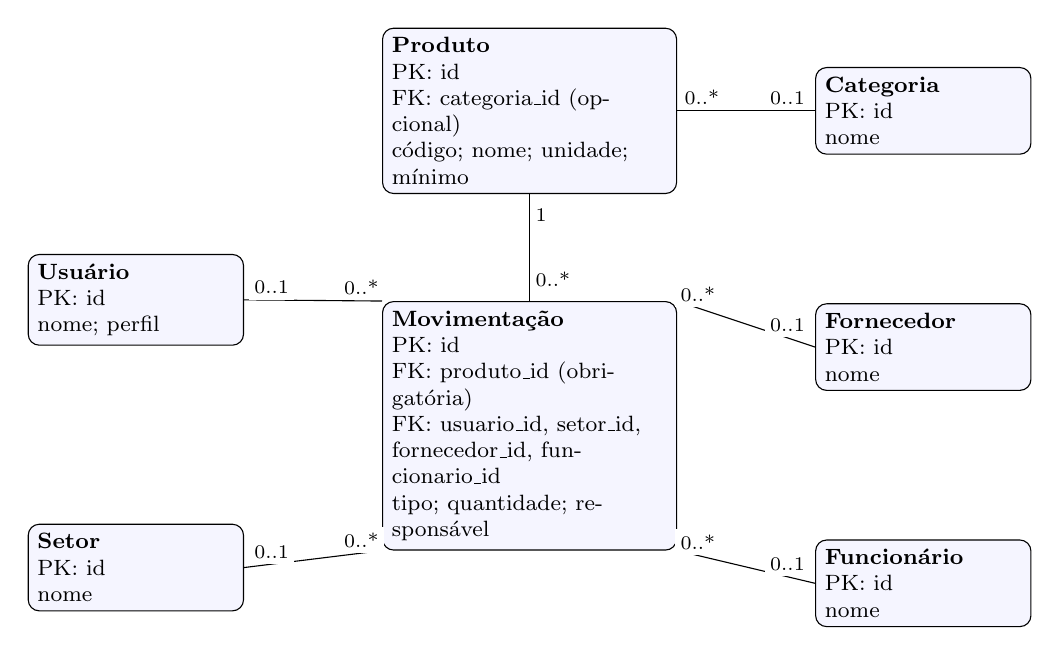
\begin{tikzpicture}[every node/.style={font=\footnotesize}, entity/.style={draw,rounded corners,align=left,text width=2.5cm,minimum height=1.1cm,fill=blue!4},card/.style={font=\scriptsize,fill=white,inner sep=2pt}]
\node[entity,text width=3.5cm] (mov) at (0,0) {\textbf{Movimentação}\\PK: id\\FK: produto\_id (obrigatória)\\FK: usuario\_id, setor\_id,\\fornecedor\_id, funcionario\_id\\tipo; quantidade; responsável};
\node[entity,text width=3.5cm] (prod) at (0,4) {\textbf{Produto}\\PK: id\\FK: categoria\_id (opcional)\\código; nome; unidade; mínimo};
\node[entity] (cat) at (5,4) {\textbf{Categoria}\\PK: id\\nome};
\node[entity] (usr) at (-5,1.6) {\textbf{Usuário}\\PK: id\\nome; perfil};
\node[entity] (set) at (-5,-1.8) {\textbf{Setor}\\PK: id\\nome};
\node[entity] (forn) at (5,1) {\textbf{Fornecedor}\\PK: id\\nome};
\node[entity] (func) at (5,-2) {\textbf{Funcionário}\\PK: id\\nome};
\draw (mov.north) -- node[card,pos=0.2,right] {0..*} node[card,pos=0.8,right] {1} (prod.south);
\draw (prod.east) -- node[card,pos=0.18,above] {0..*} node[card,pos=0.8,above] {0..1} (cat.west);
\draw (mov.north west) -- node[card,pos=0.15,above] {0..*} node[card,pos=0.8,above] {0..1} (usr.east);
\draw (mov.south west) -- node[card,pos=0.15,above] {0..*} node[card,pos=0.8,above] {0..1} (set.east);
\draw (mov.north east) -- node[card,pos=0.15,above] {0..*} node[card,pos=0.8,above] {0..1} (forn.west);
\draw (mov.south east) -- node[card,pos=0.15,above] {0..*} node[card,pos=0.8,above] {0..1} (func.west);
\end{tikzpicture}

\caption{Recorte do modelo de dados das movimentações de estoque}
\label{fig:dados-estoque}
\par\smallskip
{\footnotesize Fonte: elaboração própria a partir dos modelos em \cite{EstoqueFacilRepositorio}.}
\end{figure}

Cada movimentação referencia obrigatoriamente um produto; um produto pode possuir nenhuma ou várias movimentações. Na estrutura consultada, categoria no produto e usuário, setor, fornecedor e funcionário na movimentação são vínculos opcionais. Sua existência não comprova que toda retirada identifique o destinatário ou o usuário autenticado: o preenchimento e as regras de obrigatoriedade precisarão ser conferidos nos cenários de avaliação.

O desenho omite entidades de inventário, pedidos de reposição, lotes e empresa, além de atributos e relacionamentos secundários, para destacar o núcleo operacional. No modelo completo existem vínculos adicionais, inclusive \texttt{empresa\_id} e \texttt{lote\_id}. Não há, neste recorte, relação direta entre produto e fornecedor: a associação ilustrada ocorre por movimentação. No TCC II, atualizarei a documentação completa junto à versão final e tratarei a validação entre empresas separadamente dos vínculos de consumo por setor.

\subsection{Funções e atores em diagramas UML}
\label{sec:uml-funcoes}

Nas Figuras~\ref{fig:uml-operacao} e~\ref{fig:uml-administracao}, apresento casos de uso UML que extraí das rotas e das dependências de autorização da cópia local examinada. O limite retangular representa o sistema; os atores representam perfis, e cada elipse expressa um objetivo do usuário, não uma tela isolada. Na primeira figura, os atores são repetidos à direita para evitar cruzamentos de associações; cada par representa o mesmo perfil. As associações agrupam as capacidades principais para preservar a leitura. Por exemplo, ``gerir pedidos de reposição'' compreende gerar, ajustar quantidades, marcar como enviado, concluir e cancelar; a conclusão não registra automaticamente a entrada dos itens recebidos. O administrador também tem acesso às operações do operador e às consultas do visualizador, conforme as permissões das rotas. A variante ``administrador geral'' corresponde a um administrador sem empresa vinculada e concentra as ações globais de empresas, backup e aparência.

\begin{figure}[htb]
\centering
\resizebox{\textwidth}{!}{\begin{tikzpicture}[x=1cm,y=1cm,scale=0.89,transform shape,
  caso/.style={draw,ellipse,align=center,minimum width=3.2cm,minimum height=0.78cm,font=\scriptsize},
  ator/.style={font=\scriptsize,align=center},
  associacao/.style={thin}]
  \draw (2.5,-0.65) rectangle (14.2,8.35);
  \node[anchor=north west,font=\footnotesize\bfseries] at (2.7,8.2) {Estoque Fácil -- operação e consulta};
  \node[ator] (vis) at (1.15,6.15) {\begin{tikzpicture}[scale=.55]\draw (0,0) circle (.22);\draw (0,-.22)--(0,-.9) (-.48,-.42)--(.48,-.42) (0,-.9)--(-.42,-1.42) (0,-.9)--(.42,-1.42);\end{tikzpicture}\\Visualizador};
  \node[ator] (op) at (1.15,2.05) {
\begin{tikzpicture}[scale=.55]\draw (0,0) circle (.22);\draw (0,-.22)--(0,-.9) (-.48,-.42)--(.48,-.42) (0,-.9)--(-.42,-1.42) (0,-.9)--(.42,-1.42);\end{tikzpicture}\\Operador};
  \node[ator] (visdir) at (15.55,6.15) {
\begin{tikzpicture}[scale=.55]\draw (0,0) circle (.22);\draw (0,-.22)--(0,-.9) (-.48,-.42)--(.48,-.42) (0,-.9)--(-.42,-1.42) (0,-.9)--(.42,-1.42);\end{tikzpicture}\\Visualizador};
  \node[ator] (opdir) at (15.55,2.05) {
\begin{tikzpicture}[scale=.55]\draw (0,0) circle (.22);\draw (0,-.22)--(0,-.9) (-.48,-.42)--(.48,-.42) (0,-.9)--(-.42,-1.42) (0,-.9)--(.42,-1.42);\end{tikzpicture}\\Operador};
  \node[caso] (saldo) at (5.25,6.9) {Consultar saldo atual};
  \node[caso] (hist) at (10.65,6.9) {Consultar histórico\\de movimentações};
  \node[caso] (rel) at (5.25,5.45) {Consultar e exportar\\relatórios};
  \node[caso] (lotes) at (10.65,5.45) {Consultar lotes\\e vencimentos};
  \node[caso] (prod) at (5.25,3.8) {Manter produtos\\e importar arquivo};
  \node[caso] (entrada) at (10.65,3.8) {Registrar entrada};
  \node[caso] (saida) at (5.25,2.35) {Registrar saída para\\setor e funcionário};
  \node[caso] (xml) at (10.65,2.35) {Importar NF-e em XML};
  \node[caso] (inv) at (5.25,0.9) {Conferir inventário\\e ajustar divergências};
  \node[caso] (pedido) at (10.65,0.9) {Gerir pedidos\\de reposição};
  \foreach \n in {saldo,rel} \draw[associacao] (vis.east)--(\n.west);
  \foreach \n in {hist,lotes} \draw[associacao] (visdir.west)--(\n.east);
  \foreach \n in {prod,saida,inv} \draw[associacao] (op.east)--(\n.west);
  \foreach \n in {entrada,xml,pedido} \draw[associacao] (opdir.west)--(\n.east);
\end{tikzpicture}
}
\caption{Casos de uso UML de consulta e operação do Estoque Fácil}
\label{fig:uml-operacao}
\par\smallskip
{\footnotesize Fonte: elaboração própria a partir das rotas do protótipo disponíveis em \cite{EstoqueFacilRepositorio}.}
\end{figure}

\begin{figure}[htb]
\centering
\resizebox{\textwidth}{!}{\begin{tikzpicture}[x=1cm,y=1cm,scale=0.89,transform shape,
  caso/.style={draw,ellipse,align=center,minimum width=3.6cm,minimum height=0.78cm,font=\scriptsize},
  ator/.style={font=\scriptsize,align=center}]
  \draw (2.5,0.1) rectangle (13.8,6.65);
  \node[anchor=north west,font=\footnotesize\bfseries] at (2.7,6.5) {Estoque Fácil -- administração};
  \node[ator] (adm) at (1.1,3.25) {\begin{tikzpicture}[scale=.55]\draw (0,0) circle (.22);\draw (0,-.22)--(0,-.9) (-.48,-.42)--(.48,-.42) (0,-.9)--(-.42,-1.42) (0,-.9)--(.42,-1.42);\end{tikzpicture}\\Administrador};
  \node[ator] (geral) at (15.25,3.25) {
\begin{tikzpicture}[scale=.55]\draw (0,0) circle (.22);\draw (0,-.22)--(0,-.9) (-.48,-.42)--(.48,-.42) (0,-.9)--(-.42,-1.42) (0,-.9)--(.42,-1.42);\end{tikzpicture}\\Administrador geral};
  \node[caso] (cad) at (5.05,5.25) {Manter cadastros\\auxiliares};
  \node[caso] (usu) at (5.05,3.45) {Gerir usuários e perfis};
  \node[caso] (audit) at (5.05,1.65) {Consultar auditoria e logs};
  \node[caso] (emp) at (11.05,5.25) {Gerir empresas clientes};
  \node[caso] (backup) at (11.05,3.45) {Gerar backup};
  \node[caso] (apar) at (11.05,1.65) {Configurar aparência};
  \foreach \n in {cad,usu,audit} \draw (adm.east)--(\n.west);
  \foreach \n in {emp,backup,apar} \draw (geral.west)--(\n.east);
\end{tikzpicture}
}
\caption{Casos de uso UML de administração do Estoque Fácil}
\label{fig:uml-administracao}
\par\smallskip
{\footnotesize Fonte: elaboração própria a partir das rotas do protótipo disponíveis em \cite{EstoqueFacilRepositorio}.}
\end{figure}

Na referência examinada, o visualizador consulta produtos, saldos, movimentações, lotes, inventários, pedidos e relatórios, mas não recebe permissão para registrar alterações nesses fluxos. O operador pode cadastrar e importar produtos, efetuar entradas e saídas, confirmar importação de NF-e em XML, conduzir inventários e alterar pedidos. O administrador mantém, além disso, categorias, fornecedores, setores, funcionários e usuários, e consulta auditoria e logs. A API de leitura com token é uma interface de integração separada dos perfis de sessão e não foi representada como ator humano. O termo ``importar NF-e'' significa ler XML e registrar entradas; o sistema não emite nota fiscal.

O caso de uso ``registrar saída'' é detalhado na Figura~\ref{fig:uml-saida}. A rota exige produto, setor e funcionário ativos do mesmo contexto de empresa, valida a quantidade informada e aciona o serviço. Este bloqueia o produto, apura o saldo, recusa uma quantidade superior ao disponível e, se válida, grava a movimentação e confirma a transação. O diagrama resume o percurso principal e a alternativa de saldo insuficiente; não substitui a avaliação de concorrência prevista no protocolo. Embora as chaves \texttt{setor\_id} e \texttt{funcionario\_id} sejam anuláveis no modelo relacional, a tela de saída examinada exige ambas. No TCC II, testarei essa diferença entre regra da interface e restrição do banco por meio das rotas e dos serviços.

\begin{figure}[htb]
\centering
\resizebox{\textwidth}{!}{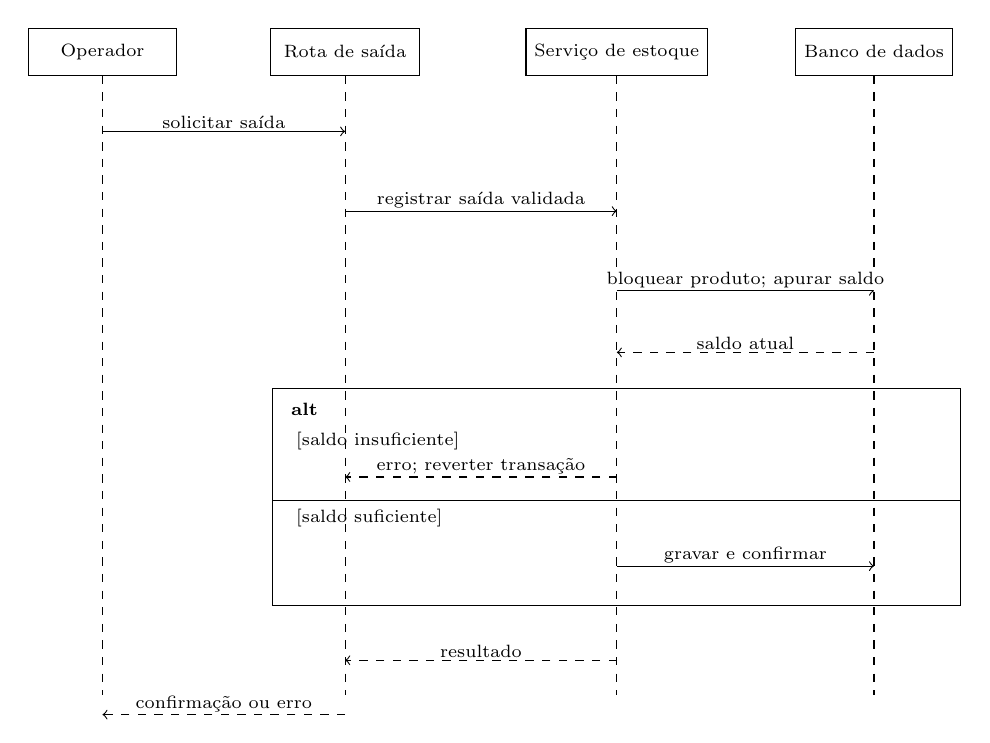
\begin{tikzpicture}[x=1cm,y=1cm,scale=0.92,transform shape,
  participante/.style={draw,rectangle,align=center,minimum width=2.05cm,minimum height=.65cm,font=\scriptsize},
  mensagem/.style={->,thin}, retorno/.style={->,thin,dashed},
  rotulo/.style={font=\scriptsize,fill=white,inner sep=1pt}]
  \node[participante] (u) at (0,9.2) {Operador};
  \node[participante] (r) at (3.35,9.2) {Rota de saída};
  \node[participante] (s) at (7.1,9.2) {Serviço de estoque};
  \node[participante] (b) at (10.65,9.2) {Banco de dados};
  \foreach \n in {u,r,s,b} \draw[dashed] (\n.south)--++(0,-8.55);
  \draw[mensagem] (0,8.1)--node[rotulo,above]{solicitar saída} (3.35,8.1);
  \draw[mensagem] (3.35,7.0)--node[rotulo,above]{registrar saída validada} (7.1,7.0);
  \draw[mensagem] (7.1,5.9)--node[rotulo,above]{bloquear produto; apurar saldo} (10.65,5.9);
  \draw[retorno] (10.65,5.05)--node[rotulo,above]{saldo atual} (7.1,5.05);
  \draw (2.35,4.55) rectangle (11.85,1.55);
  \node[anchor=north west,font=\scriptsize\bfseries] at (2.48,4.48) {alt};
  \node[anchor=west,font=\scriptsize] at (2.55,3.83) {[saldo insuficiente]};
  \draw[retorno] (7.1,3.33)--node[rotulo,above]{erro; reverter transação} (3.35,3.33);
  \draw (2.35,3.0)--(11.85,3.0);
  \node[anchor=west,font=\scriptsize] at (2.55,2.76) {[saldo suficiente]};
  \draw[mensagem] (7.1,2.1)--node[rotulo,above]{gravar e confirmar} (10.65,2.1);
  \draw[retorno] (7.1,.8)--node[rotulo,above]{resultado} (3.35,.8);
  \draw[retorno] (3.35,.05)--node[rotulo,above]{confirmação ou erro} (0,.05);
\end{tikzpicture}
}
\caption{Diagrama de sequência UML para registrar uma saída de estoque}
\label{fig:uml-saida}
\par\smallskip
{\footnotesize Fonte: elaboração própria a partir de \path{app/routes/estoque_routes.py} e \path{app/services/estoque_service.py} disponíveis em \cite{EstoqueFacilRepositorio}.}
\end{figure}

Esses casos de uso descrevem funcionalidades presentes no código, ainda sem comprovação de atendimento em testes. Curva ABC, apuração contábil do estoque e cálculo do tempo de armazenamento não foram identificados como funções implementadas nas rotas examinadas; permanecem candidatos a requisitos futuros, dependentes de regras de classificação, custo e data de entrada. Assim, não aparecem nas figuras como capacidades entregues.

\section{Origem exploratória da demanda}

Minha experiência no suporte a um ERP em Sinop constitui a origem empírica inicial da questão de pesquisa. Nesse contexto profissional, percebi situações de contagens frequentes para esclarecer saldos e dificuldades de consulta a quantidades, tempo de armazenamento, valores contábeis e classificação por curva ABC. Registro essa percepção retrospectivamente, sem levantamento sistemático de organizações, frequência, período de observação ou instrumentos de coleta. Por isso, utilizo-a para motivar e formular hipóteses de necessidade, e não como resultado de entrevista, levantamento de campo ou estimativa de prevalência entre pequenas e médias empresas.

Na análise documental e bibliográfica, confrontarei essas percepções com práticas de controle descritas em fontes identificáveis. Na matriz de requisitos, cada demanda receberá origem explícita: minha observação exploratória, fonte bibliográfica, documentação de produto, regra operacional ou decisão de projeto. No TCC II, avaliarei o vínculo de retirada a setor e funcionário no escopo definido. Tempo de armazenamento, contabilidade de estoque e curva ABC permanecerão candidatos a investigação complementar, pois dependem de definições de dados, período, custo e finalidade de uso ainda não estabelecidas para a versão avaliada.

Não identificarei nem descreverei como participante da pesquisa nenhuma empresa que atendi durante minha atividade profissional. Eventual validação das necessidades com organizações exigirá procedimento de coleta próprio, nos termos da seção de aspectos éticos. Essa separação permite aproveitar a experiência que motivou o trabalho sem atribuir ao relato a força de evidência obtida por pesquisa de campo.

\section{Questões operacionais e evidências}

Desdobro a questão geral em três questões operacionais:
\begin{enumerate}
    \item quais necessidades percebi e quais regras documentadas justificam os requisitos selecionados para o sistema?
    \item como as decisões arquiteturais e tecnológicas atendem a esses requisitos, e quais limitações introduzem?
    \item em que medida a versão avaliada atende aos critérios funcionais e de qualidade estabelecidos no protocolo?
\end{enumerate}

Responderei à primeira questão por meio de fichas de fontes e da matriz de requisitos; à segunda, pela descrição da arquitetura e pelos registros de decisão; e à terceira, pelos casos de teste, medições e registros de falhas. Com essa organização, poderei identificar a evidência que sustenta cada conclusão, inclusive quando um requisito não puder ser verificado.

\section{Levantamento bibliográfico e documental}

Realizarei uma revisão bibliográfica narrativa orientada pelos temas gestão de estoques, sistemas de informação, engenharia de requisitos, arquitetura web, qualidade de produto e avaliação de software. Consultarei Google Acadêmico, SciELO e repositórios institucionais para localização de trabalhos, além de publicações de organismos de normalização e documentação oficial das tecnologias. O procedimento não será apresentado como revisão sistemática ou exaustiva.

Nas buscas, combinarei expressões em português e inglês, como ``gestão de estoques'' e ``sistema web'', ``inventory management'' e ``information system'', e ``software quality'' e ``case study''. Para cada busca, registrarei a base, a data, a expressão utilizada e os documentos selecionados. Obras conceituais serão admitidas independentemente do ano; para tecnologias e normas, a edição deverá ser identificada e compatível com a discussão.

Incluirei fontes com autoria ou responsabilidade institucional identificável, conteúdo acessível e relação direta com o problema. Excluirei documentos duplicados, materiais sem procedência verificável e textos cujo conteúdo disponível não permita sustentar a afirmação pretendida. Em uma ficha de leitura, reunirei referência, objetivo, conceito aproveitado, limitação e seção do TCC em que a fonte será utilizada. Na redação, privilegiarei sínteses próprias e citações associadas às afirmações que as fontes efetivamente sustentam.

\section{Levantamento de soluções e identificação de demandas}

No levantamento documental inicial, contemplo Bling, Conta Azul Pro, Omie, Odoo Inventory e ERPNext, com fontes oficiais consultadas em 16 de setembro de 2026 e síntese apresentada na Seção~\ref{sec:mercado}. Atualizarei a análise antes da avaliação final, preservando a data e as condições de cada consulta. Outras soluções poderão ser incorporadas se possuírem controle de entradas e saídas, interface web e documentação pública suficiente para aplicar os mesmos critérios. A seleção será intencional e não probabilística; a disponibilidade de documentação será reconhecida como fator que limita a composição da amostra.

Examinarei cada solução quanto a cadastros, movimentações, histórico, conferência de estoque, relatórios, permissões, integrações e condições de implantação documentadas. Registrarei versão ou edição, endereço consultado, data de acesso e eventuais dependências de módulos ou planos. Preços somente serão utilizados se necessários à análise e associados à data e às condições anunciadas.

Classificarei cada característica como: documentada como disponível, documentada com restrição, explicitamente não oferecida na edição consultada ou não verificada. Ausência de menção não será interpretada como ausência do recurso. Facilidade de uso e desempenho não serão inferidos de páginas comerciais ou de documentação. Quando uma informação depender de acesso não disponível, a limitação será registrada.

Examinarei os diferenciais propostos na Seção~\ref{sec:diferenciais} por cenários de consumo interno, execução do fluxo sem venda associada, reconstrução do ambiente e alteração rastreável de uma regra. A comparação documental não será utilizada para alegar exclusividade de um recurso não verificado nos concorrentes.

Tratarei as funções recorrentes como candidatas a requisitos. Sua adoção dependerá da pertinência ao problema, das regras do domínio e da viabilidade no período do TCC. Necessidades atribuídas especificamente a empresas do norte de Mato Grosso somente poderão ser afirmadas a partir de evidências dessas organizações; a comparação de produtos, isoladamente, não fornecerá essa validação regional.

\section{Especificação e priorização dos requisitos}

No processo de especificação, adotarei identificação, critérios de aceitação e rastreabilidade, em consonância com as práticas de requisitos apresentadas no SWEBOK \cite{SWEBOK2026}. Em cada item, registrarei origem, descrição, regra associada, prioridade, dependências, estado de implementação e testes relacionados. Os estados serão: proposto, implementado sem verificação, aprovado em teste, reprovado e não avaliado.

A prioridade será essencial quando o requisito for necessário ao fluxo de cadastro, movimentação e consulta segura; importante quando ampliar a conferência e o acompanhamento; e desejável quando puder ser adiado sem inviabilizar o núcleo. Na Tabela~\ref{tab:requisitos}, defino o conjunto inicial para orientar a execução. Seus critérios representam compromissos de verificação, não resultados já obtidos.

\begin{table}[htb]
\centering
\caption{Requisitos funcionais iniciais e critérios de aceitação}
\label{tab:requisitos}
\small
\begin{tabular}{p{0.09\textwidth}p{0.24\textwidth}p{0.56\textwidth}}
\hline
\textbf{ID} & \textbf{Requisito} & \textbf{Critério de aceitação} \\ \hline
RF01 & Autenticar e autorizar & Recusar acesso não autenticado e operações incompatíveis com o perfil. \\ \hline
RF02 & Manter cadastros & Validar campos obrigatórios, identificar produtos e preservar vínculos de registros inativados. \\ \hline
RF03 & Registrar entrada & Acrescentar a quantidade ao saldo e registrar produto, data e responsável. \\ \hline
RF04 & Registrar saída & Aceitar quantidade positiva até o saldo e recusar excesso sem alterar os registros. \\ \hline
RF05 & Consultar saldo e histórico & Apresentar valores compatíveis com as movimentações e os filtros aplicados. \\ \hline
RF06 & Gerar relatórios & Produzir relatório e exportação com os mesmos dados e filtros da consulta correspondente. \\ \hline
\end{tabular}
\par\smallskip
{\footnotesize Fonte: elaboração própria para o protocolo de avaliação.}
\end{table}

Classifico RF01 a RF05 como essenciais e RF06 como importante. Especificarei os requisitos não funcionais por cenários, como preservação da consistência sob duas saídas simultâneas, rejeição de operação sem permissão e reconstrução do ambiente com a versão documentada. Limites de desempenho dependerão do ambiente de referência e serão registrados antes das medições; sem limite previamente definido, a análise será descritiva, sem classificação arbitrária de aprovação.

\section{Projeto, desenvolvimento e implantação}

Na análise arquitetural, mapearei rotas, serviços, modelos e templates, verificando como uma operação percorre essas partes. O modelo de dados deverá explicitar entidades, chaves, relacionamentos e regras de integridade. Para cada decisão relevante, registrarei contexto, alternativas, justificativa, consequências e requisito atendido. Na documentação, distinguirei organização prevista e estrutura observada no código.

No TCC II, desenvolverei incrementos relacionados aos requisitos priorizados. Registrarei cada demanda em uma \textit{issue}, farei a implementação em branch específica e a submeterei por \textit{pull request} à branch \texttt{developer}. A revisão e as verificações automatizadas deverão preceder a promoção para \texttt{main}. Como acumularei os papéis de desenvolvedor e pesquisador, declararei quando eu mesmo realizar a implementação e a revisão, sem caracterizar essa revisão como independente.

Empregarei o GitHub Actions para organizar verificações, construção e publicação de imagens, conforme os recursos descritos em sua documentação \cite{GitHubActionsDocs,GitHubContainerRegistry}. A configuração consultada ainda referencia \texttt{develop} no gatilho, e não demonstra uma etapa dedicada de testes. A adequação à branch \texttt{developer} e a inclusão das verificações serão tarefas do desenvolvimento, com evidência de execução antes de serem consideradas concluídas.

Utilizarei Docker Compose para organizar o ambiente experimental \cite{DockerComposeDocs}. Configurarei PostgreSQL tanto no desenvolvimento usado para os testes quanto na homologação, com bancos e volumes separados. Como a aplicação admite SQLite por padrão em execução local, verificarei e registrarei a configuração efetiva antes de cada coleta. Os ensaios utilizarão dados sintéticos e não executarão operações destrutivas em produção.

\section{Protocolo de avaliação}
\label{sec:protocolo}

Na avaliação do TCC II, empregarei um recorte do modelo de qualidade de produto da ISO/IEC 25010:2023 \cite{ISO25010_2023}. A escolha das dimensões decorre do risco de operações incorretas, acesso indevido e perda de registros no domínio de estoques. Em cada execução, registrarei requisito, caso de teste, versão, pré-condições, entradas, resultado esperado, resultado obtido, evidência e conclusão. Casos bloqueados serão distinguidos dos aprovados e reprovados.

\subsection{Preparação do ambiente e dos dados}

Registrarei sistema operacional, processador, memória, versões do Python e do PostgreSQL, dependências, imagem de contêiner, navegador, configuração de rede e recursos atribuídos aos serviços. Uma base sintética terá produtos, categorias, fornecedores e usuários nos perfis necessários. O script de criação e sua semente, quando houver geração pseudoaleatória, serão preservados para reconstrução dos cenários.

Para verificar a correção funcional, utilizarei uma base pequena com saldos previamente conhecidos. Para desempenho, prepararei dois conjuntos propostos: mil produtos com dez mil movimentações e dez mil produtos com cem mil movimentações. Esses volumes são parâmetros experimentais, sem pretensão de representar uma empresa específica. Alterações necessárias por restrição de recursos serão justificadas e registradas antes da coleta definitiva.

\subsection{Adequação funcional e integridade}

Incluirei nos testes operações válidas, entradas inválidas e condições de fronteira. Um caso básico partirá de saldo zero, registrará uma entrada de dez unidades e uma saída de três, esperando saldo sete. Em seguida, tentará uma saída de oito unidades, que deverá ser recusada sem alterar saldo ou histórico. Também serão verificadas quantidades nulas ou negativas, campos obrigatórios ausentes e referências inexistentes, conforme o tipo de operação.

O teste de concorrência iniciará com cinco unidades e duas solicitações simultâneas de saída de quatro. O resultado esperado será uma única confirmação e saldo final um. A execução deverá comprovar sobreposição das operações, por sincronização das requisições e registro dos eventos; apenas enviar chamadas sequenciais não verificará o cenário. Falhas serão documentadas e novamente testadas após correção.

Calcularei a proporção de aprovação $P = N_a/N_e \times 100$, em que $N_a$ é o número de casos aprovados e $N_e$ o número de casos executados. Se nenhum caso for executado, o indicador será não calculável. Também apresentarei números absolutos de casos planejados, bloqueados e não executados, evitando que a taxa esconda lacunas. O conjunto essencial somente será considerado atendido quando todos os seus critérios forem aprovados; a taxa global não compensará falhas de saldo ou autorização.

\subsection{Eficiência de desempenho}

Medirei operações de consulta de produtos, consulta de saldo, registro de movimentação e geração de relatório. Cada cenário combinará um dos volumes definidos com um ou cinco usuários virtuais, usando a mesma sequência de operações. Haverá cinco execuções de aquecimento, excluídas da análise, e trinta observações medidas por operação e cenário. Para escritas, a base será restaurada ou as entradas serão controladas para manter condições comparáveis.

Medirei o tempo no cliente entre o envio da requisição HTTP e o recebimento completo da resposta, com identificação da ferramenta e de sua versão. Esse tempo não será apresentado como duração de renderização no navegador. Informarei mediana, mínimo, máximo, percentil 95 e taxa de erros, com preservação dos dados brutos. O percentil será calculado pelo método do posto mais próximo, posição $\lceil 0{,}95n \rceil$ na amostra ordenada. Respostas com falha serão contabilizadas separadamente e não descartadas sem registro.

As trinta observações fornecerão uma caracterização exploratória; não serão utilizadas para afirmar capacidade máxima, estabilidade prolongada ou desempenho de todas as instalações. Sem ensaio equivalente das soluções de mercado, seus tempos não serão comparados aos do Estoque Fácil.

\subsection{Segurança e confiabilidade}

No roteiro de segurança, selecionarei requisitos aplicáveis do OWASP ASVS 5.0.0, mantendo os identificadores completos e as justificativas de inclusão \cite{OWASPASVS2025}. Verificarei rejeição de acesso sem sessão, permissões por perfil, encerramento de sessão, tratamento de entradas e proteção das operações de alteração. Também testarei o acesso por URL direta além da navegação pelos menus. Se houver operação multiempresa, registros de uma empresa sintética não deverão ser consultados ou alterados por usuário de outra.

Para confiabilidade, observarei os efeitos de uma falha controlada durante a gravação e da reinicialização do serviço após uma transação confirmada. O primeiro cenário deverá preservar o estado anterior ou concluir integralmente a operação; o segundo deverá conservar os registros confirmados. Caso o backup integre a versão avaliada, a cópia será restaurada em banco isolado e conferida por contagens, identificadores e saldos. A existência do arquivo de backup não será tomada como comprovação de recuperação.

\subsection{Interação e manutenibilidade}

Na inspeção da interface, verificarei navegação por teclado, identificação dos campos, mensagens de validação, confirmação de operações e acesso a tabelas nas larguras de 360, 768 e 1366 pixels. No registro, incluirei navegador, tarefa, problema identificado e captura de tela. Esses resultados serão relatados como inspeção técnica. A distinção entre inspeção e usabilidade em contexto de uso seguirá a definição da ISO 9241-11:2018 \cite{ISO9241_11}; satisfação e facilidade percebida não serão inferidas sem usuários.

Examinarei a manutenibilidade por inspeção da localização das regras, duplicações relevantes, dependências entre módulos e correspondência entre alterações e testes. Uma alteração delimitada em regra de validação será acompanhada desde o requisito até sua verificação, registrando os módulos afetados e eventuais regressões. O número de arquivos alterados será interpretado em seu contexto, sem funcionar isoladamente como nota de qualidade.

\section{Análise dos dados e apresentação dos resultados}

Organizarei os dados qualitativos por categorias: necessidade, requisito, decisão, evidência e limitação. Na análise, confrontarei documentação, código e comportamento observado, registrando divergências. Por exemplo, uma função anunciada no README, mas não executável no ambiente de teste, será apresentada com essa restrição, sem ser automaticamente classificada como atendida.

Apresentarei os dados quantitativos por cenário, com contagens e estatísticas descritivas. Na discussão, explicarei quais requisitos foram atendidos, quais falharam e quais permaneceram sem evidência. Após correções, os resultados anteriores serão preservados e associados à versão correspondente. O estudo não atribuirá causalmente melhoria de qualidade a uma tecnologia sem um desenho de comparação que sustente essa conclusão.

Na comparação documental com outras soluções, utilizarei os mesmos critérios e distinguirei recursos anunciados de recursos verificados por execução. Sua finalidade será situar o escopo e as limitações do Estoque Fácil. Como produto final da análise, apresentarei matriz de requisitos, registros de decisões, relatório de testes e síntese das limitações e possibilidades de evolução.

\section{Reprodutibilidade e ameaças à validade}

Preservarei o identificador da versão, diferenças locais relevantes, arquivos de configuração sem segredos, dependências, scripts de dados, casos de teste, logs e medições brutas. Imagens de contêiner serão identificadas por etiqueta e, quando disponível, por resumo criptográfico. Documentos externos serão registrados com endereço, edição e data de acesso. Esses materiais permitirão reconstruir as condições descritas, respeitando as restrições de acesso ao repositório.

Na discussão de validade, seguirei a preocupação com planejamento e transparência do estudo de caso destacada por \citeonline{RunesonHost2009}. Neste projeto, reconheço como ameaças principais meu duplo papel de desenvolvedor e avaliador, a escolha intencional das soluções comparadas, o uso de dados sintéticos e a avaliação de uma única aplicação. Critérios prévios, manutenção dos resultados negativos e revisão pelo orientador reduzirão interpretações favoráveis não sustentadas.

As métricas selecionadas cobrem apenas parte da qualidade do produto. Tempos de resposta não representam satisfação, e aprovação em cenários funcionais não demonstra ausência de defeitos. Limitarei as conclusões à versão, ao ambiente e aos casos executados. A generalização será analítica, pela discussão das decisões e de suas condições de aplicação, sem extrapolação estatística para empresas ou usuários da região.

\section{Aspectos éticos e tratamento das informações}

O protocolo principal utiliza documentos, código e dados sintéticos, sem recrutamento de participantes ou importação de bases reais de clientes. Revisarei logs e capturas de tela para evitar divulgação de credenciais, tokens e informações pessoais. Restringirei os testes de acesso ao ambiente experimental autorizado.

Uma eventual etapa com entrevistas, questionários ou tarefas realizadas por usuários exigirá protocolo complementar, com objetivo, seleção dos participantes, instrumentos, consentimento e tratamento dos dados definidos antes da coleta, observadas as exigências institucionais aplicáveis. Essa etapa não integra os resultados previstos como já disponíveis. Na sua ausência, as conclusões permanecerão limitadas à análise documental e à avaliação técnica descritas neste capítulo.
